% !TeX spellcheck = fr_FR
\chapter{Chapitre 1 : Données ATLAS}

Les données ATLAS, au cœur de cette étude, proviennent de la plateforme Open Transport Data Swiss [\ref{ref:open_transport_data_swiss}]. Cette ressource centralise les données des transports publics en Suisse, offrant une base précieuse pour l’analyse et le développement d’applications.\\
\textit{Sauf indication contraire, toutes les statistiques et cartes de ce chapitre sont calculées sur le snapshot de données du 11 août 2025.}

\medskip
\noindent\textbf{Reproductibilité.} Sauf mention contraire, toutes les figures et statistiques de ce chapitre ont été produites par des scripts reproductibles disponibles sous \texttt{memoire/scripts\_used/}. Nous n’indiquons plus les scripts individuellement dans les légendes afin d’alléger la lecture.

\section{Arrêts}

La section sur les arrêts s’appuie sur le jeu de données traffic-points-actual-date [\ref{ref:traffic_points_actual_date}]. Ce jeu de données recense les arrêts de transport public en Suisse, avec des informations détaillées sur leur localisation et leurs caractéristiques. Ces points peuvent être visualisés sur une carte interactive via l’application web https://atlas.app.sbb.ch/ [\ref{ref:atlas_app_sbb}], offrant une représentation graphique intuitive des arrêts.

Nous nous concentrons ici sur deux colonnes principales : le numéro et la désignation des arrêts.

Le numéro d’un arrêt correspond à la référence UIC (Union Internationale des Chemins de fer), un standard international permettant d’identifier les lieux de transport public. Les deux premiers chiffres représentent le code du pays ; la Suisse, par exemple, utilise le code 85[\ref{ref:wikipedia_uic_codes}]. Ainsi, un numéro UIC comme "8502034" désigne un arrêt spécifique du réseau suisse.

La colonne "désignation" fait référence à une identification locale : une valeur de "3" peut, par exemple, indiquer que l’arrêt correspond à la plateforme 3 d’une gare.

Enfin, les données incluent également des informations sur l’opérateur responsable de chaque arrêt, un élément potentiellement utile pour établir des correspondances avec d’autres jeux de données.

Le jeu de données distingue deux types de \texttt{trafficPointElementType} : \texttt{BOARDING\_AREA} et \texttt{BOARDING\_PLATFORM}. Notre analyse se limite aux \texttt{BOARDING\_PLATFORM}, car les \texttt{BOARDING\_AREA} ne disposent pas de coordonnées géographiques. Pour extraire ces informations, nous avons développé un script Python, \texttt{get\_atlas\_data.py}. Extrait simplifié du chargement/filtrage:

\begin{codebox}[language=Python]{Extrait — \texttt{get\_atlas\_stops}}
def get_atlas_stops(output_path, download_url):
    response = requests.get(download_url)
    response.raise_for_status()
    with zipfile.ZipFile(io.BytesIO(response.content)) as z:
        csv_filename = z.namelist()[0]
        with z.open(csv_filename) as f:
            df = pd.read_csv(f, sep=';')
            # Suisse (UIC pays = 85) et coordonnees valides (WGS84)
            df = df[df['uicCountryCode'] == 85]
            df = df.dropna(subset=['wgs84North', 'wgs84East'])
            # Comptage des quais
            boarding_platforms = df[df['trafficPointElementType'] == 'BOARDING_PLATFORM']
            df.to_csv(output_path, sep=';', index=False)
\end{codebox}



\paragraph{Statistiques ATLAS (WGS84).} Sur l’instantané analysé :
\begin{itemize}
  \item \textbf{Lignes avec coordonnées}: \textit{56\,510}.
  \item \textbf{\texttt{BOARDING\_PLATFORM}}: \textit{55\,818}.
  \item \textbf{UIC distincts (\texttt{number})}: \textit{27\,225}.
  \item \textbf{\texttt{designation} non vides}: \textit{11\,462} (\textit{109} valeurs distinctes).
  \item \textbf{\texttt{designation} manquantes}: \textit{44\,356}, dont \textit{4\,499} cas où l’unique entrée du \texttt{number} est sans désignation.
  \item \textbf{Entrées identifiables par (\texttt{number}, \texttt{designation}) seul}: \textit{10\,928}.
  \item \textbf{Total identifiables par \texttt{number} + (\texttt{designation} ou unicité du \texttt{number})}: \textit{15\,427}.
\end{itemize}

\begin{figure}[h]
  \centering
  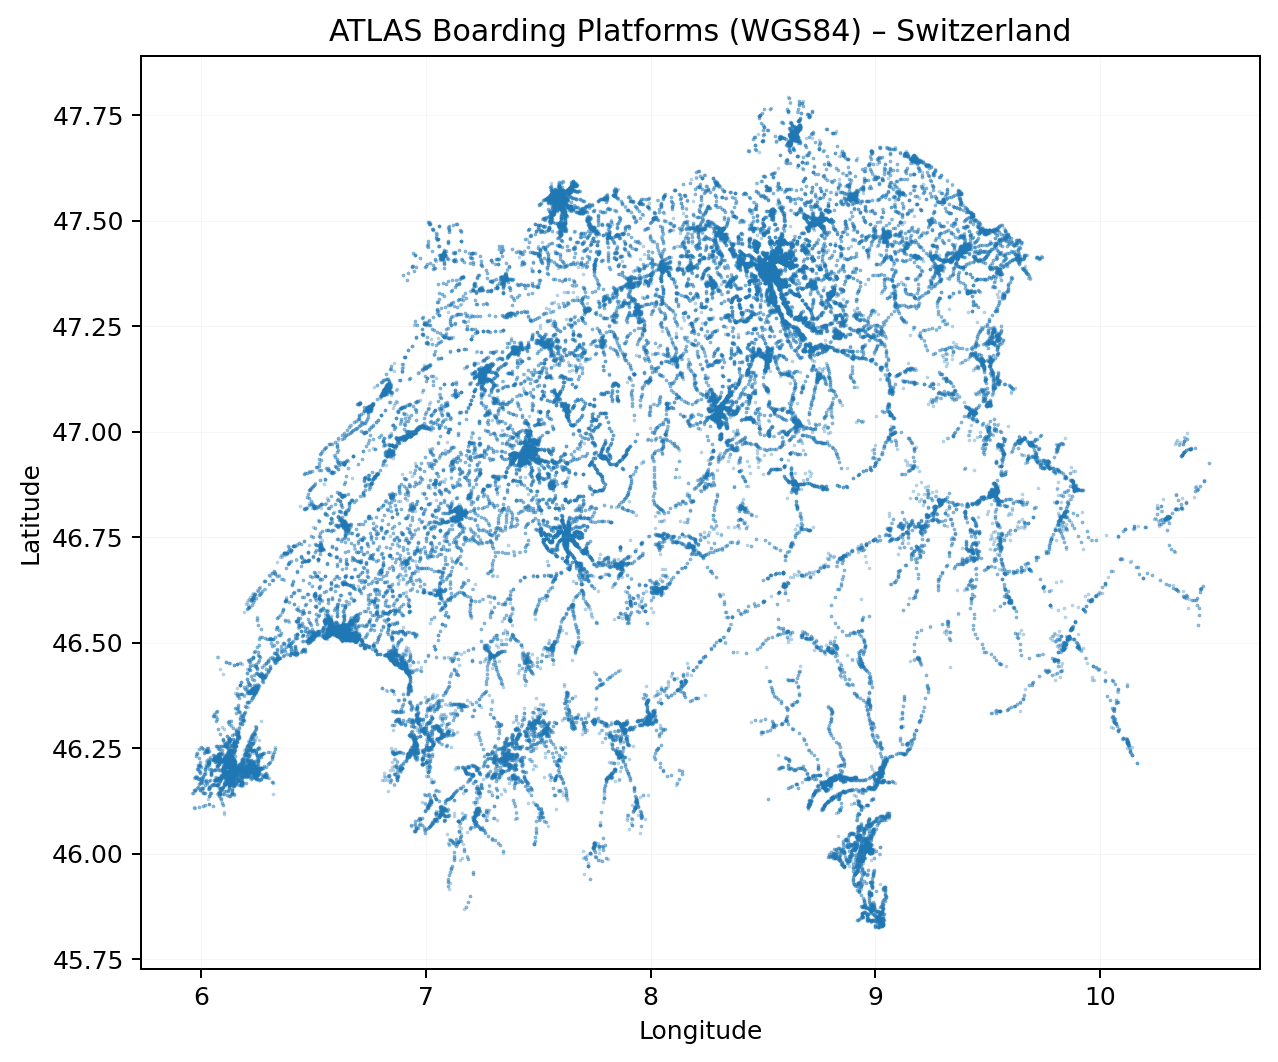
\includegraphics[width=.76\linewidth]{figures/plots/atlas_points_switzerland.png}
  \caption[ATLAS BOARDING\_PLATFORM: distribution nationale]{ATLAS \texttt{BOARDING\_PLATFORM}: distribution nationale (WGS84).}
  \label{fig:atlas_ch_points}
\end{figure}

\begin{figure}[h]
  \centering
  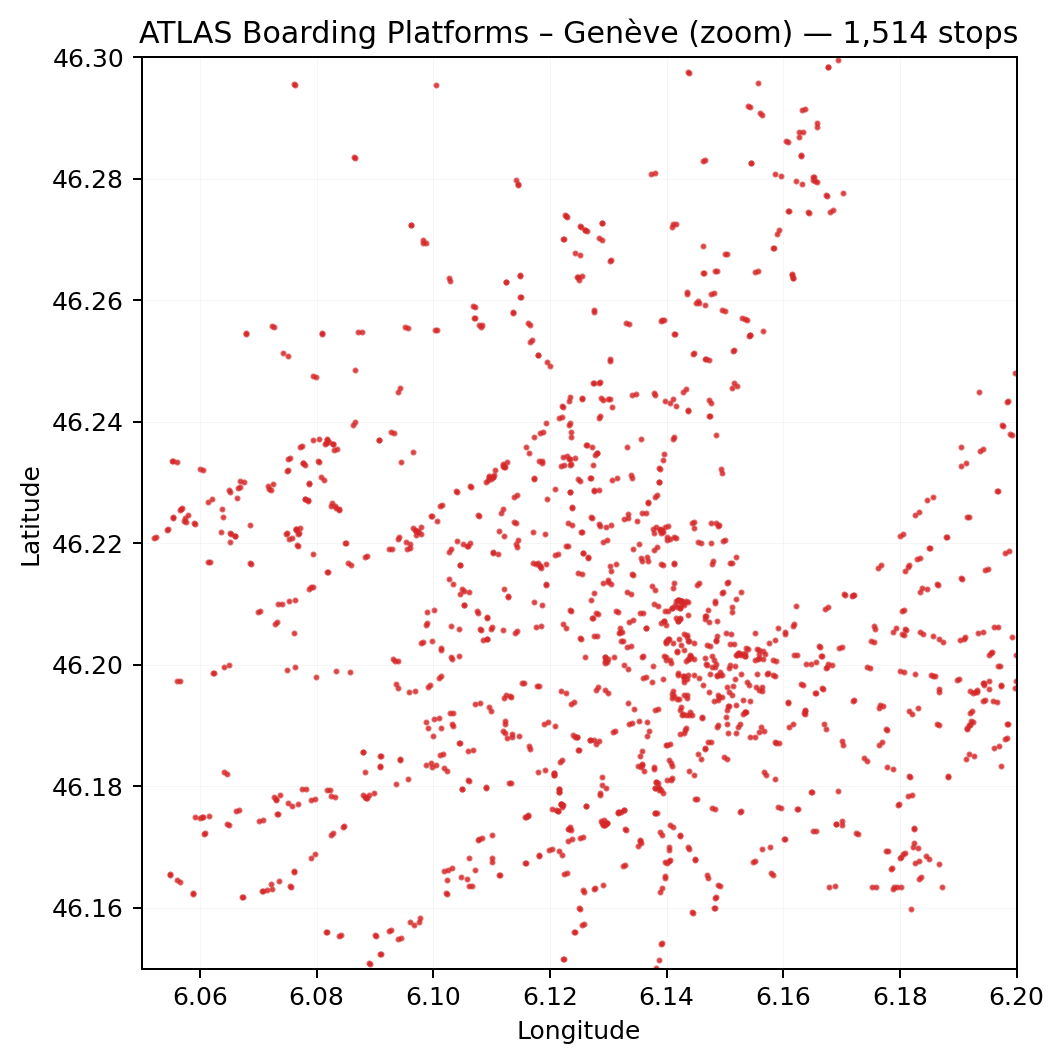
\includegraphics[width=.6\linewidth]{figures/plots/atlas_points_geneva.png}
  \caption[ATLAS BOARDING\_PLATFORM: Genève]{ATLAS \texttt{BOARDING\_PLATFORM}: zoom sur Genève.}
  \label{fig:atlas_geneva}
\end{figure}

\begin{figure}[h]
  \centering
  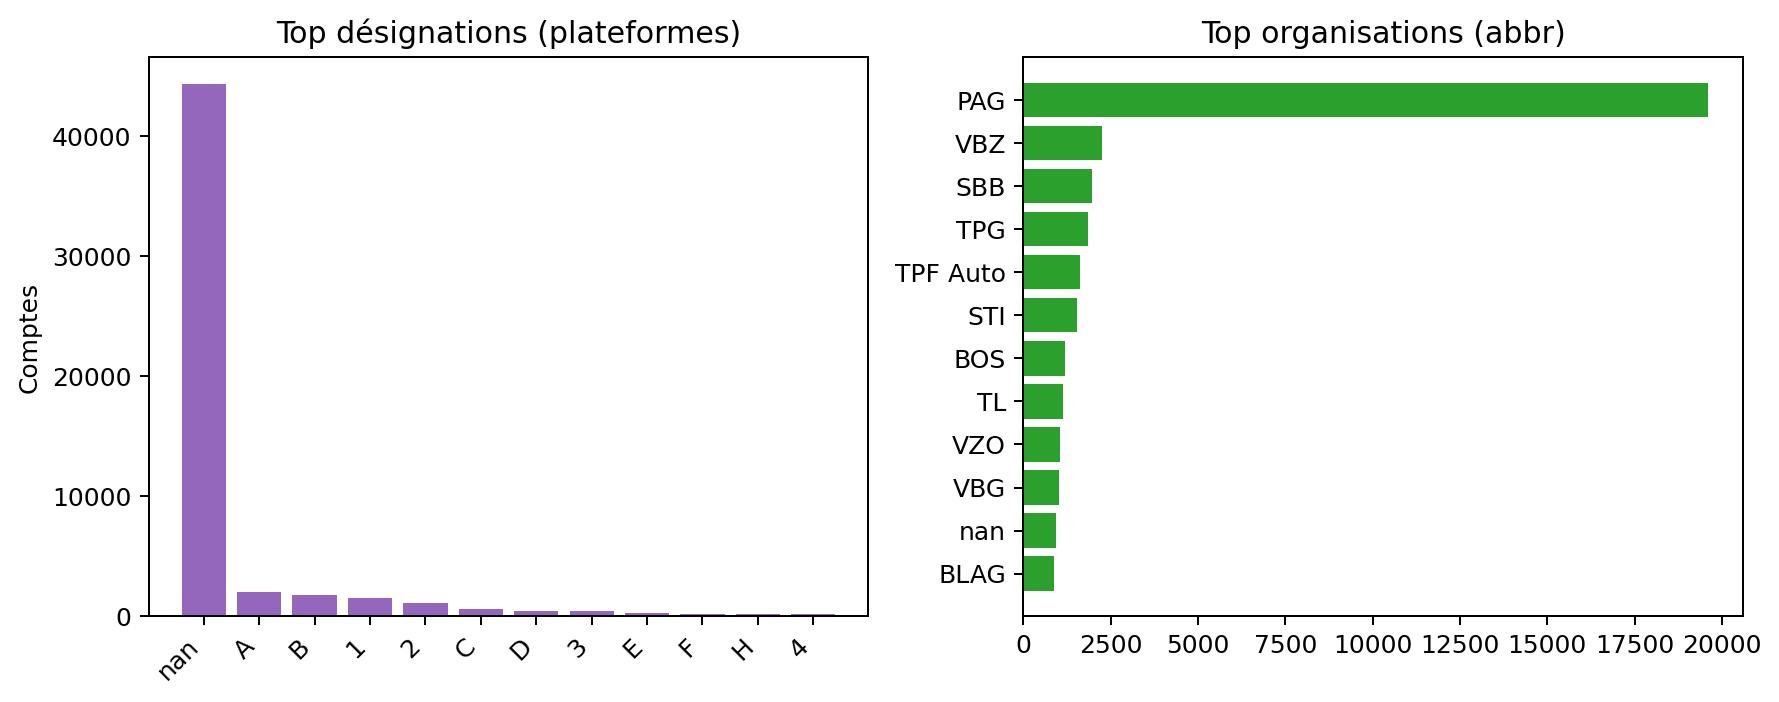
\includegraphics[width=.85\linewidth]{figures/plots/atlas_designation_operators.png}
  \caption[Désignations et opérateurs ATLAS]{À gauche: désignations de plateforme les plus fréquentes (hors valeurs manquantes). À droite: principales organisations (abrégés) déclarées.}
  \label{fig:atlas_distribs}
\end{figure}

\noindent\textit{Remarque.} Les valeurs manquantes de \texttt{designation} (très nombreuses) sont exclues du top pour éviter un effet disproportionné. Comme indiqué plus haut, \(10\,928\) entrées sont déjà identifiables par le couple \((\texttt{number},\texttt{designation})\) et \(4\,499\) supplémentaires sont uniques par \texttt{number} seul.

Ce script filtre les données pour ne conserver que les entrées \texttt{BOARDING\_PLATFORM} avec des coordonnées valides.

Concernant les coordonnées, le fichier fournit deux systèmes : le système de référence suisse LV95 et le système de référence global WGS84. Étant donné que les données d'OpenStreetMap (OSM) utilisent les coordonnées WGS84, nous nous concentrerons uniquement sur cet ensemble de coordonnées pour le moment.

\section{GTFS}

Le General Transit Feed Specification (GTFS) est un format d’échange numérique initié par Google pour standardiser les horaires des transports publics et leurs informations géographiques, telles que la localisation des arrêts. En Suisse, ces données sont fournies par les entreprises de transport et publiées sur la plateforme OpenTransportDataSuisse. Elles servent à développer des applications pratiques, comme les outils de consultation d’horaires ou de planification de trajets.

Bien que notre projet se focalise actuellement sur la synchronisation des arrêts, les données GTFS relatives aux trajets suscitent également notre intérêt. Elles pourraient faciliter la correspondance entre les arrêts ATLAS et ceux d’OpenStreetMap, en exploitant les informations sur les itinéraires présentes dans les deux ensembles de données. Parmi les nombreux fichiers GTFS disponibles, quatre retiennent notre attention : \texttt{stops.txt}, \texttt{stop\_times.txt}, \texttt{routes.txt} et \texttt{trips.txt}.

\subsection{Description des fichiers}

Les fichiers GTFS suivants sont cruciaux pour notre analyse :

\begin{itemize}
    \item \textbf{\texttt{stops.txt}} : Ce fichier répertorie les arrêts avec leurs coordonnées géographiques et d’autres attributs. 
    Un extrait est présenté dans le tableau \ref{tab:stops}.
    \item \textbf{\texttt{routes.txt}} : Il décrit les lignes de transport, avec des informations comme le nom court, le nom long, et le type de transport. 
    Voir le tableau \ref{tab:routes}.
    \item \textbf{\texttt{trips.txt}} : Ce fichier associe les trajets aux lignes et aux services.
    Un exemple est donné dans le tableau \ref{tab:trips}.
    \item \textbf{\texttt{stop\_times.txt}} : Il contient les horaires d’arrivée et de départ pour chaque arrêt d’un trajet.
    Voir le tableau \ref{tab:stop_times}.
    \begin{table}[h]
    \caption{Extrait du fichier \texttt{stops.txt}}
    \label{tab:stops}
    \centering
    \begin{tabular}{l l r r l l}
    \toprule
    stop\_id & stop\_name & stop\_lat & stop\_lon  & parent\_station \\
    \midrule
    1101064 & Malpensa Aeroporto, terminal 1 & 45.6272 & 8.7111 & \\
    8000339 & Weissenhorn Eschach & 48.3010 & 10.1351  & \\
    8000709:0:2 & Neckarsulm Mitte & 49.1935 & 9.2229  & \\
    8000778 & Asselheim (D) & 49.5762 & 8.1616  & \\
    8000781 & Grünstadt-Nord & 49.5734 & 8.1708 & \\
    8000988 & Witzighausen & 48.3174 & 10.0978 & \\
    8002015 & Nördlingen & 48.8508 & 10.4979 & 8002015P \\
    8002015:0:4 & Nördlingen & 48.8509 & 10.4979 & 8002015P \\
    \bottomrule
    \end{tabular}
    \end{table}

    \begin{table}[h]
    \caption{Extrait du fichier \texttt{routes.txt}}
    \label{tab:routes}
    \centering
    \begin{tabular}{l l l l l l}
    \toprule
    route\_id & agency\_id & route\_short\_name & route\_desc & route\_type \\
    \midrule
    91-10-A-j22-1 & 37 & 10 & T & 900 \\
    91-10-B-j22-1 & 78 & S10 & S & 109 \\
    91-10-C-j22-1 & 11 & S10 & S & 109 \\
    91-10-E-j22-1 & 65 & S10 & S & 109 \\
    91-10-F-j22-1 & 11 & RE10 & RE & 106 \\
    91-10-G-j22-1 & 11 & SN10 & SN & 109 \\
    91-10-j22-1 & 3849 & 10 & T & 900 \\
    91-10-Y-j22-1 & 82 & IR & IR & 103 \\
    \bottomrule
    \end{tabular}
    \end{table}

    \begin{table}[h]
    \caption{Extrait du fichier \texttt{trips.txt}}
    \label{tab:trips}
    \centering
    \begin{tabular}{l l l l l l l l l}
    \toprule
    route\_id & trip\_id & trip\_short\_name & direction\_id  \\
    \midrule
    91-8-H-j25-1  & 994.TA.91-8-H-j25-1.59.R  & 6278 & 1 \\
    91-8-H-j25-1  & 995.TA.91-8-H-j25-1.59.R  & 2978 & 1 \\
    91-8-H-j25-1  & 996.TA.91-8-H-j25-1.59.R & 2787 & 1 \\
    91-8-H-j25-1  & 997.TA.91-8-H-j25-1.59.R  & 4879 & 1 \\
    91-8-H-j25-1  & 998.TA.91-8-H-j25-1.59.R  & 10407 & 1 \\
    91-8-H-j25-1  & 999.TA.91-8-H-j25-1.59.R  & & 1 & \\
    \bottomrule
    \end{tabular}
    \end{table}

    \begin{table}[h]
    \caption{Extrait du fichier \texttt{stop\_times.txt}}
    \label{tab:stop_times}
    \centering
    \begin{tabular}{l l l l r l l}
    \toprule
    trip\_id & arrival\_time & departure\_time & stop\_id & stop\_sequence \\
    \midrule
    1.TA.1-9-j17-1.1.H & 05:25:00 & 05:25:00 & 8502034:0:2 & 1 \\
    1.TA.1-9-j17-1.1.H & 05:28:00 & 05:29:00 & 8502033:0:2 & 2 \\
    1.TA.1-9-j17-1.1.H & 05:33:00 & 05:33:00 & 8502032:0:1 & 3 \\
    1.TA.1-9-j17-1.1.H & 05:36:00 & 05:36:00 & 8502031:0:1 & 4 \\
    1.TA.1-9-j17-1.1.H & 05:42:00 & 05:42:00 & 8502030:0:2 & 5 \\
    1.TA.1-9-j17-1.1.H & 05:50:00 & 05:50:00 & 8502119:0:7 & 6 \\
    2.TA.1-9-j17-1.2.H & 05:53:00 & 05:53:00 & 8502034:0:1 & 1 \\
    2.TA.1-9-j17-1.2.H & 05:57:00 & 05:58:00 & 8502033:0:2 & 2 \\
    \bottomrule
    \end{tabular}
    \end{table}
\end{itemize}


\subsection{Analyse et défis de jointure}

Dans le script \texttt{get\_atlas\_data.py},nous avons crée un fichier \texttt{routes\_atlas.csv} qui associe les arrêts aux routes et directions qu’ils desservent à partir des données GTFS. On commence pour joindre les fichiers GTFS. Cette jointure s’appuie sur le fichier \texttt{stop\_times.txt} pour connecter les arrêts aux trajets via \texttt{trip\_id}, puis les trajets aux routes via \texttt{route\_id}, en extrayant des paires uniques de route-direction par arrêt, accompagnées des noms des routes.

La mise en correspondance entre la colonne \texttt{stop\_id} du fichier \texttt{stops.txt} (GTFS) et l’identifiant \texttt{sloid} d’ATLAS présente des défis significatifs. Premièrement, il n’existe pas de lien direct entre ces deux identifiants. Deuxièmement, les coordonnées géographiques des arrêts diffèrent entre les deux ensembles de données.

\textbf{Exemple 1 : "Lancy-Pont-Rouge":}
\newline
Considérons la gare "Lancy-Pont-Rouge", opérée par les CFF. Dans le fichier \texttt{stops.txt} de GTFS, les données sont les suivantes :

\begin{table}[h]
\caption{Extrait de \texttt{stops.txt} pour "Lancy-Pont-Rouge"}
\label{tab:stops_lancy_2}
\centering
\begin{tabular}{l l r r l l}
\toprule
\texttt{stop\_id} & \texttt{stop\_name} & \texttt{stop\_lat} & \texttt{stop\_lon} & \texttt{parent\_station} \\
\midrule
8516155:0:1 & Lancy-Pont-Rouge & 46.18596197 & 6.12483039 & Parent8516155 \\
8516155:0:2 & Lancy-Pont-Rouge & 46.18595575 & 6.12495615 & Parent8516155 \\
\bottomrule
\end{tabular}
\end{table}

Dans le fichier \texttt{traffic-points-actual-data}, on trouve :

\begin{table}[h]
\caption{Extrait de \texttt{traffic-points-actual-data} pour "Lancy-Pont-Rouge"}
\label{tab:traffic_lancy_2}
\centering
\begin{tabular}{l l l l r r l}
\toprule
\texttt{sloid} & \texttt{number} & \texttt{des.} & \texttt{wgs84East} & \texttt{wgs84North} & \texttt{designationOfficial} \\
\midrule
...:16155:1:1 & 8516155 & 1  & 6.12483137 & 46.18596333 & Lancy-Pont-Rouge \\
...:16155:1:2 & 8516155 & 2  & 6.12495213 & 46.18595284 & Lancy-Pont-Rouge \\
\bottomrule
\end{tabular}
\end{table}

Ici, le format de \texttt{stop\_id} dans GTFS est \texttt{uic\_number:0:local\_ref}, où \texttt{uic\_number} correspond à la colonne \texttt{number} dans ATLAS (8516155), et \texttt{local\_ref} à \texttt{designation} (1 ou 2). Cela permet une correspondance, bien que les coordonnées géographiques divergent légèrement.

\textbf{Exemple 2 : "Lausanne Bourdonnette":}
\newline
Prenons un deuxième exemple avec "Lausanne Bourdonnette". Dans \texttt{stops.txt} :
\begin{table}[h]
\caption{Extrait de \texttt{stops.txt} pour "Lausanne Bourdonnette"}
\label{tab:stops_bourdonnette_2}
\centering
\begin{tabular}{l l r r}
\toprule
\texttt{stop\_id} & \texttt{stop\_name} & \texttt{stop\_lat} & \texttt{stop\_lon} \\
\midrule
8501210:0:10000 & Lausanne, Bourdonnette & 46.52342565 & 6.59074161 \\
8501210:0:10001 & Lausanne, Bourdonnette & 46.52329585 & 6.58987025 \\
8501210:0:A & Lausanne, Bourdonnette & 46.52326494 & 6.58980736 \\
8501210:0:B & Lausanne, Bourdonnette & 46.52318459 & 6.58978940 \\
8501210:0:C & Lausanne, Bourdonnette & 46.52272720 & 6.58913363 \\
8501210:0:D & Lausanne, Bourdonnette & 46.52338238 & 6.59138840 \\
\bottomrule
\end{tabular}
\end{table}

Et dans \texttt{traffic-points-actual-data} :

\begin{table}[h]
\caption{Extrait de \texttt{traffic-points-actual-data} pour "Lausanne Bourdonnette"}
\label{tab:traffic_bourdonnette_2}
\centering
\begin{tabular}{l l l l r r l}
\toprule
\texttt{sloid} & \texttt{number} & \texttt{des.
}  & \texttt{wgs84East} & \texttt{wgs84North} & \texttt{designationOfficial} \\
\midrule
...:1210:0:1600 & 8501210 &  & 6.59074107 & 46.52342597 & Lausanne, Bourdonnette \\
...:1210:0:1610 & 8501210 &  & 6.58986994 & 46.52329351 & Lausanne, Bourdonnette \\
...:1210:0:1616 & 8501210 & B & 6.58979344 & 46.52318499 & Lausanne, Bourdonnette \\
...:1210:0:2597 & 8501210 & D & 6.59138793 & 46.52338108 & Lausanne, Bourdonnette \\
...:1210:0:2542 & 8501210 & C & 6.58913042 & 46.52272550 & Lausanne, Bourdonnette \\
\bottomrule
\end{tabular}
\end{table}

Dans ce cas, les désignations dans GTFS incluent "A", "B", "C", "D", ainsi que des références numériques comme "10000" et "10001", mais dans ATLAS,  "A" n’a pas d’équivalent direct, et les références numériques ne sont pas assignées (lignes avec \texttt{designation} vide). Les coordonnées géographiques diffèrent également.

\subsection{Résulats}
Nous générons un fichier intégré \texttt{atlas\_routes\_gtfs.csv} listant, par \texttt{sloid}, les couples \texttt{(route\_id, direction\_id)}. Sur notre jeu:
\begin{itemize}
  \item \textbf{SLOIDs couverts par GTFS}: \textit{32\,248--32\,249}.
  \item \textbf{Médiane des lignes par SLOID (GTFS)}: \textit{2}.
\end{itemize}

\begin{figure}[h]
  \centering
  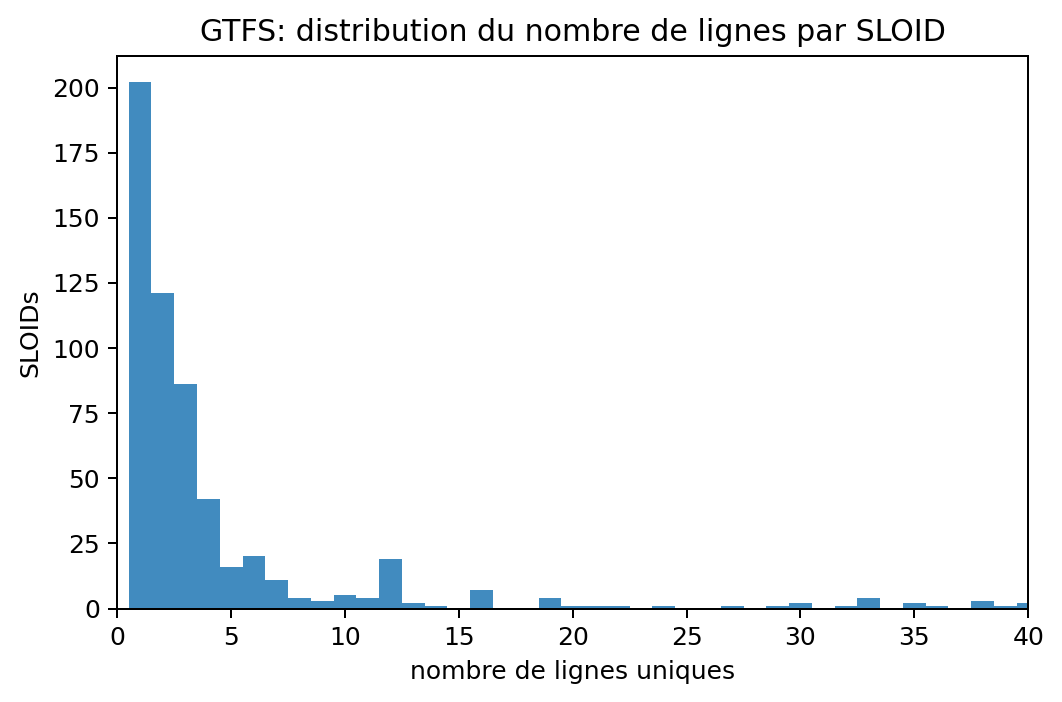
\includegraphics[width=.7\linewidth]{figures/plots/gtfs_routes_per_sloid.png}
  \caption[GTFS: lignes par SLOID]{GTFS: distribution du nombre de lignes par SLOID.}
  \label{fig:gtfs_lines_per_sloid}
\end{figure}

\noindent
Motivation: ces couples route/direction sont une brique essentielle de notre \textit{route matching} OSM (détaillé au Chapitre~4).

\subsection{Compléments cartographiques}
\begin{figure}[h]
  \centering
  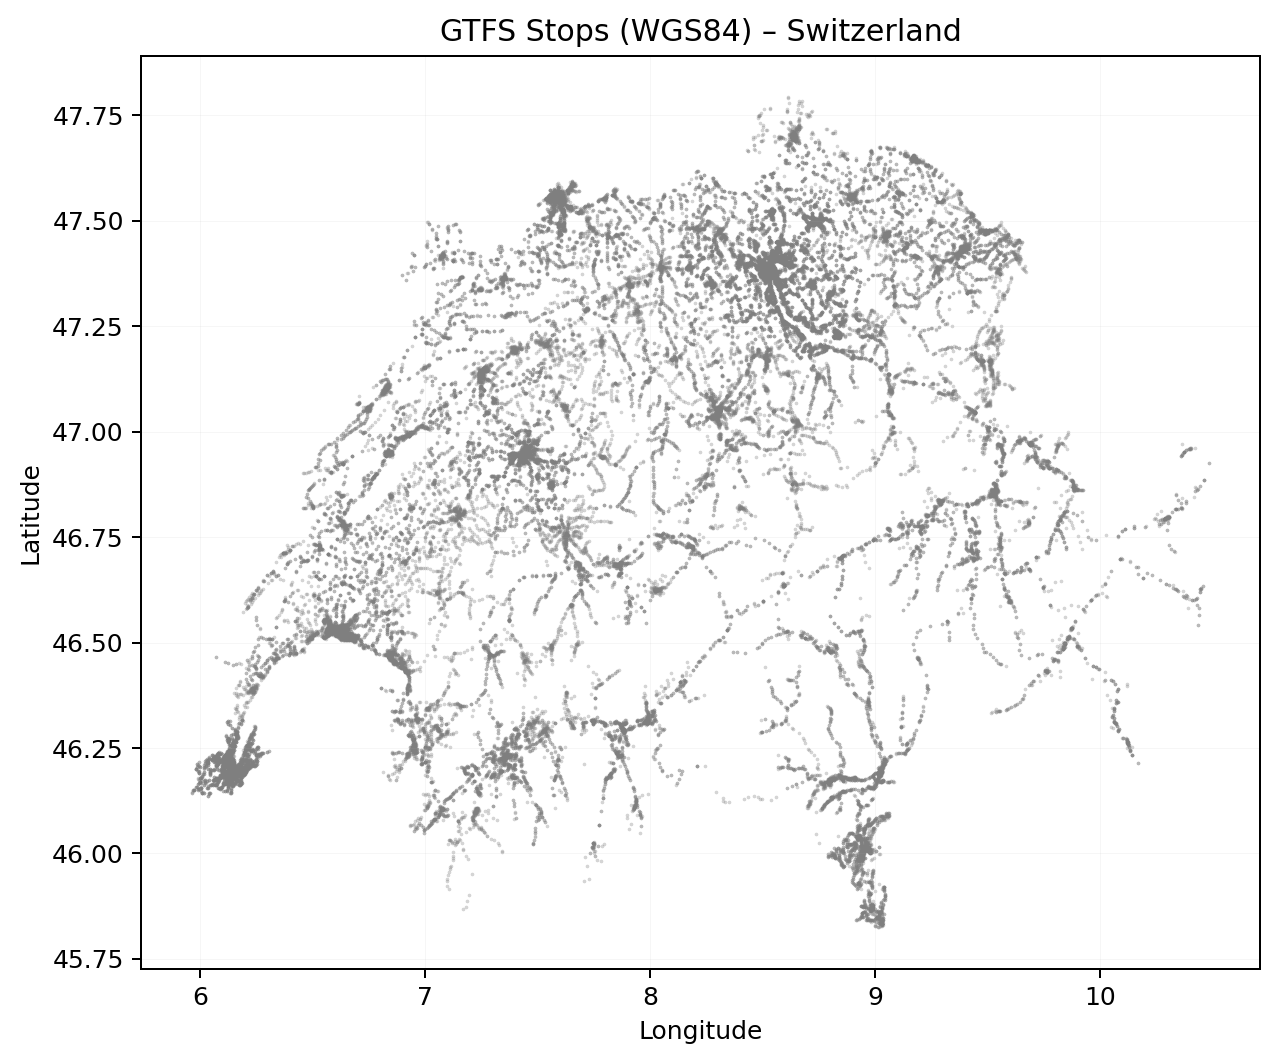
\includegraphics[width=.76\linewidth]{figures/plots/gtfs_points_switzerland.png}
  \caption[Arrêts GTFS (Suisse)]{Arrêts GTFS (Suisse): \(47\,829\) arrêts suisses détectés.}
  \label{fig:gtfs_ch_points}
\end{figure}

\begin{figure}[h]
  \centering
  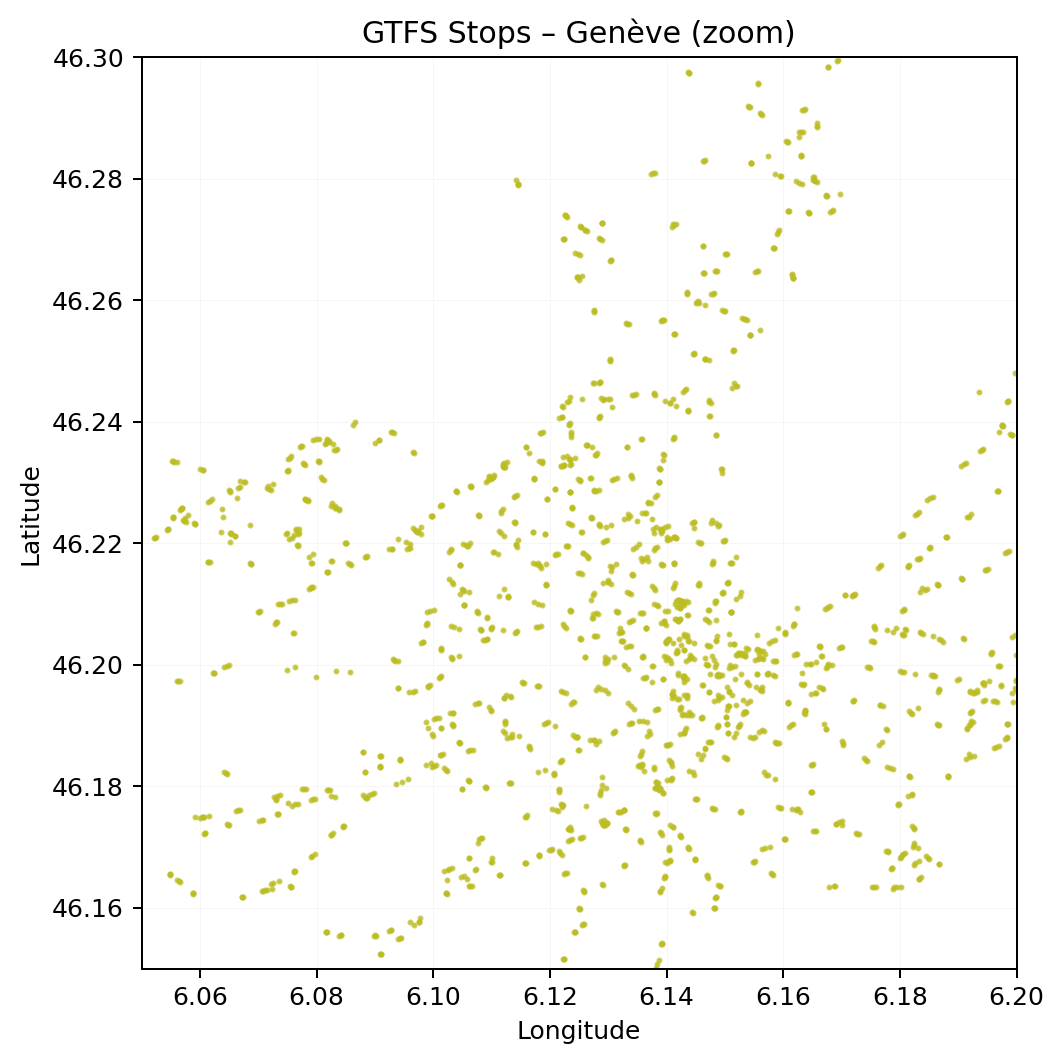
\includegraphics[width=.6\linewidth]{figures/plots/gtfs_points_geneva.png}
  \caption[Arrêts GTFS (Genève)]{Arrêts GTFS: zoom sur Genève.}
  \label{fig:gtfs_geneva}
\end{figure}

\paragraph{Distances ATLAS–GTFS: définition et interprétation.} Pour chaque \texttt{UIC} présent dans les deux jeux de données, nous calculons (i) le centroïde des arrêts GTFS associés et (ii) le centroïde des plateformes ATLAS correspondantes, puis la distance entre ces deux centroïdes. La médiane empirique de cette distance est \textbf{\(\sim 11{,}9\,m\)} (\(53\,912\) UIC considérés), ce qui atteste d’une compatibilité géométrique globale satisfaisante. Les valeurs extrêmes reflètent principalement des différences de modélisation (positionnement des plateformes vs. points d’arrêt agrégés) et des cas de gares étendues.

\begin{figure}[h]
  \centering
  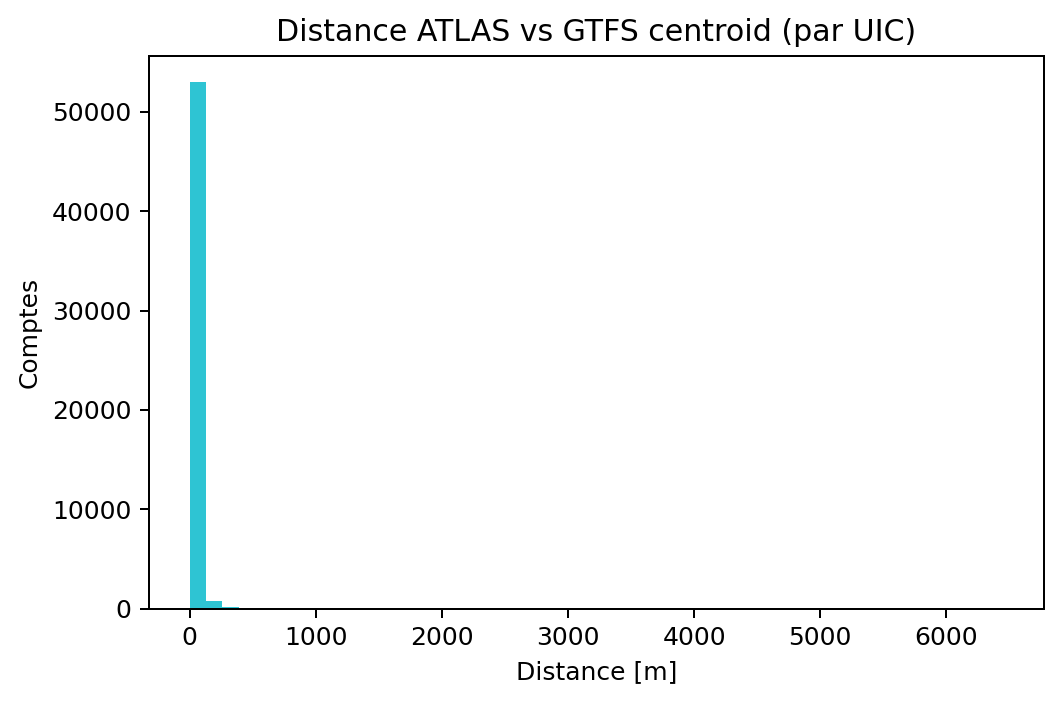
\includegraphics[width=.76\linewidth]{figures/plots/atlas_vs_gtfs_distance_hist.png}
  \caption[Distances ATLAS–GTFS par UIC]{Distribution des distances ATLAS \(\leftrightarrow\) centroïde GTFS par UIC (mètres).}
  \label{fig:atlas_gtfs_distance}
\end{figure}

\paragraph{Lecture du graphique.} La figure ci-dessus présente l’histogramme de ces distances. Les petites distances dominent (alignement global), tandis que la queue lourde correspond à des gares complexes et à des divergences de granularité.
Pour surmonter ces défis, nous avons exploité la structure de : \newline
\texttt{stop\_id} dans GTFS (\texttt{uic\_number:0:local\_ref}). \newline
Nous utilisons les colonnes \texttt{number} et \texttt{designation} d’ATLAS pour établir une correspondance avec \texttt{uic\_number} et \texttt{local\_ref}, respectivement. La référence locale (\texttt{local\_ref}) est normalisée (ex. "10000" devient "1", "10001" devient "2") pour obtenir \texttt{normalized\_local\_ref}. Les règles de correspondance sont les suivantes :

Associer si \texttt{uic\_number} (GTFS) = \texttt{number} (ATLAS) et \texttt{normalized\_local\_ref} = \texttt{designation}.
Si plusieurs entrées ATLAS existent pour un même \texttt{uic\_number} :
Associer à la seule entrée si elle est unique.
Sinon, vérifier si \texttt{normalized\_local\_ref} = \texttt{designation} ou \texttt{normalized\_local\_ref} = dernière partie de \texttt{sloid} (ex. "ATLAS:8500010:1" → "1").
Par exemple :

Pour "Lancy-Pont-Rouge", \texttt{stop\_id} "8516155:0:1" donne \texttt{uic\_number} "8516155" et \texttt{normalized\_local\_ref} "1", correspondant à \texttt{number} "8516155" et \texttt{designation} "1".
Pour "Lausanne Bourdonnette", \texttt{stop\_id} "8501210:0:B" donne \texttt{uic\_number} "8501210" et \texttt{normalized\_local\_ref} "B", correspondant à \texttt{number} "8501210" et \texttt{designation} "B".
Pour un \texttt{stop\_id} "8500030:0:2" avec plusieurs entrées ATLAS, si \texttt{sloid} "ATLAS:8500030:2" existe, il est associé car "2" correspond à \texttt{normalized\_local\_ref}.

Voici deux exemples concrets de correspondance :

GTFS : \texttt{stop\_id="8505113:0:4"}, nom "Altdorf UR", \texttt{uic\_number="8505113"}, \texttt{normalized\_local\_ref="4"} ; ATLAS : \texttt{sloid="ch:1:sloid:5113:2:4"}, nom "Altdorf UR", \texttt{number="8505113"}, \texttt{designation="4"} (match via \texttt{designation}).
GTFS : \texttt{stop\_id="8592669:0:C"}, nom "Carouge GE, Armes", \texttt{uic\_number="8592669"}, \texttt{normalized\_local\_ref="C"} ; ATLAS : \texttt{sloid="ch:1:sloid:92669:0:241732"}, nom "Carouge GE, Armes", \texttt{number="8592669"}, \texttt{designation="C"} (match via \texttt{designation}, malgré \texttt{sloid} différent).

\section{HRDF}
Le \textit{HAFAS Raw Data Format} structure des horaires exhaustifs. Deux fichiers sont clés: \texttt{BHFART} (SLOIDs gare/quai) et \texttt{GLEISE\_WGS/LV95} (infrastructure et coordonnées de quai).

\subsection{Comment nous le lisons}
Notre extraction s’effectue en deux passes efficaces et ciblées:
\begin{enumerate}
  \item \textbf{GLEISE\_LV95 \(\to\) paires (UIC, \#ref) par \texttt{sloid}.} Nous parcourons \texttt{GLEISE\_LV95} pour associer chaque \texttt{sloid} de quai au \texttt{UIC} de gare et au numéro de référence (\#ref) qui identifie le quai.
  \item \textbf{FPLAN \(\to\) directions.} Pour ces \((\text{UIC}, \#\text{ref})\) cibles seulement, nous analysons \texttt{FPLAN} afin d’extraire, par voyage, le premier et le dernier arrêt. En reliant ces arrêts à leurs noms (via \texttt{BAHNHOF}), nous formons des chaînes directionnelles \textit{noms} (\enquote{Genève \(\to\) Lausanne}) et \textit{UIC} (\enquote{8501008 \(\to\) 8501120}).
\end{enumerate}

\noindent Ces chaînes seront utilisées au Chapitre~4 pour améliorer le \textit{route matching} en absence d’identifiants de direction GTFS directement disponibles sur OSM.

\begin{codebox}[language=Python]{Extraits — parsing ciblé HRDF}
def parse_gleise_lv95_for_sloids(hrdf_path, target_sloids):
    # Associer chaque sloid cible a (UIC, #ref), en un premier passage rapide
    ...

def extract_fplan_directions_for_trips(hrdf_path, target_trip_keys):
    # Pour les trajets cibls, recuperer premier/dernier arret et le nom de ligne
    ...
\end{codebox}

\subsection{Informations exploitées}
\begin{itemize}
  \item \textbf{SLOID de quai} et position (WGS84);
  \item \textbf{Chaînes directionnelles} \textit{nom} (\textit{Genève} \(\to\) \textit{Lausanne}) et \textit{UIC} (\(8501008 \to 8501120\)).
\end{itemize}

\subsection{Statistiques clés}
\begin{cmdbox}
\# SLOIDs de quai (GLEISE\_LV95)
grep -o "g A ch:1:sloid:[^[:space:]]\\+" data/raw/GLEISE_LV95 | \\
  sed 's/^g A //' | sort -u | wc -l
30935

\# SLOIDs de quai dans BHFART ("G a" = quai, "G A" = gare)
grep -o "G a ch:1:sloid:[^[:space:]]\\+" data/raw/BHFART | sed 's/^G a //' | sort -u | wc -l
30935
grep -o "G A ch:1:sloid:[^[:space:]]\\+" data/raw/BHFART | sed 's/^G A //' | sort -u | wc -l
31913

\# Toutes occurrences (gare+quai)
grep -o "ch:1:sloid:[^[:space:]]\\+" data/raw/BHFART | sort -u | wc -l
62848
\end{cmdbox}

\noindent
Après extraction (\texttt{atlas\_routes\_hrdf.csv}) : \textbf{\(28\,757\)} SLOIDs couverts ; médiane des directions (noms) par SLOID : \textbf{4}. Ces chaînes \enquote{nom} et \enquote{UIC} enrichissent les correspondances quand un identifiant de direction explicite n’est pas disponible côté OSM.

\begin{figure}[h]
  \centering
  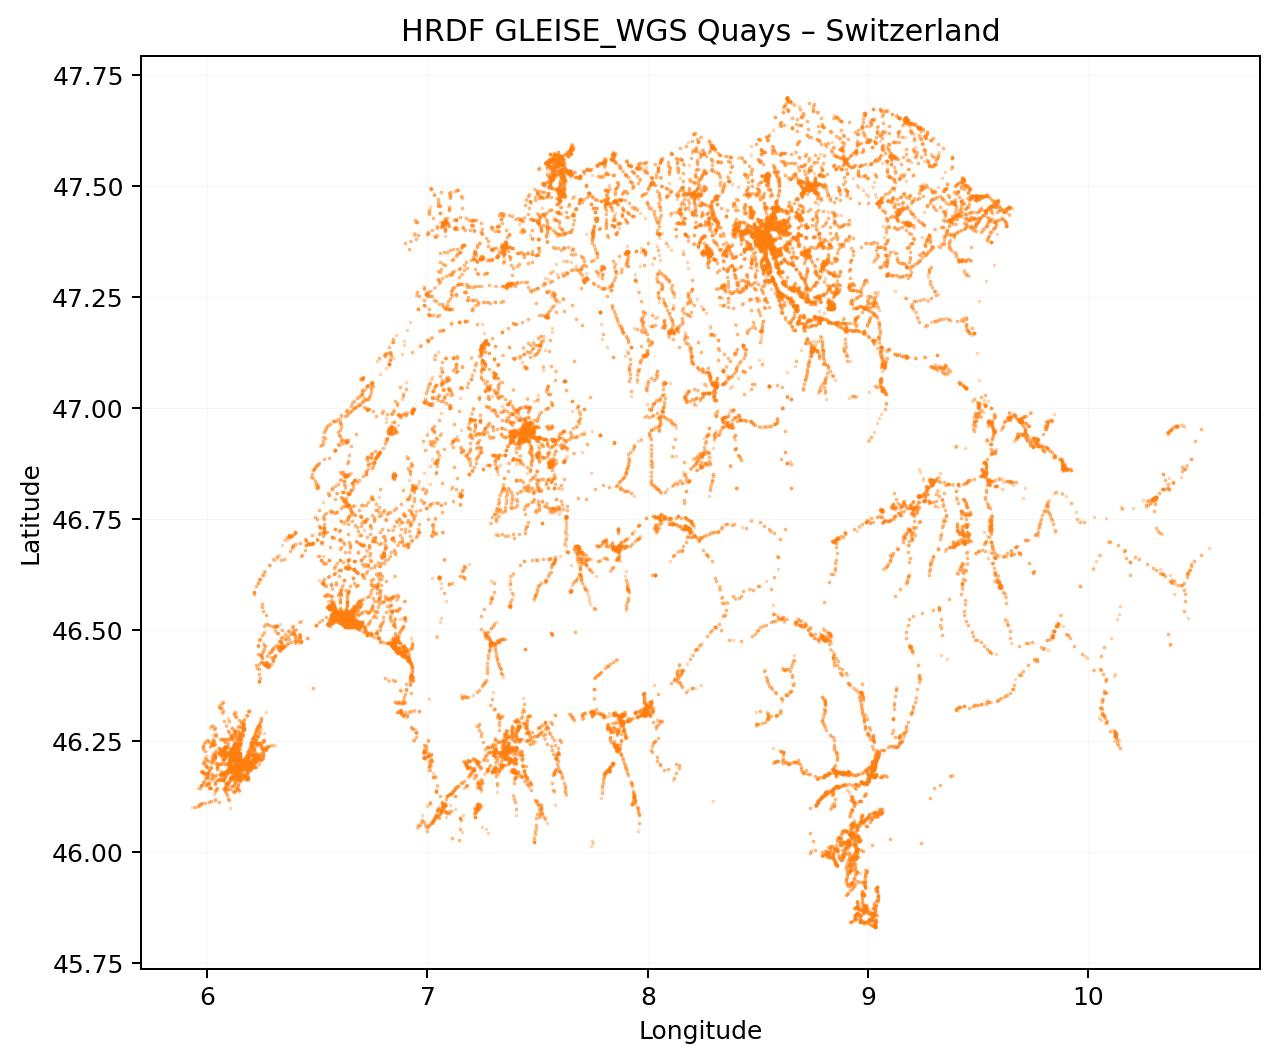
\includegraphics[width=.76\linewidth]{figures/plots/hrdf_quays_switzerland.png}
  \caption[Quais HRDF – Suisse]{Quais HRDF (\texttt{GLEISE\_WGS}) – Suisse.}
\end{figure}

\begin{figure}[h]
  \centering
  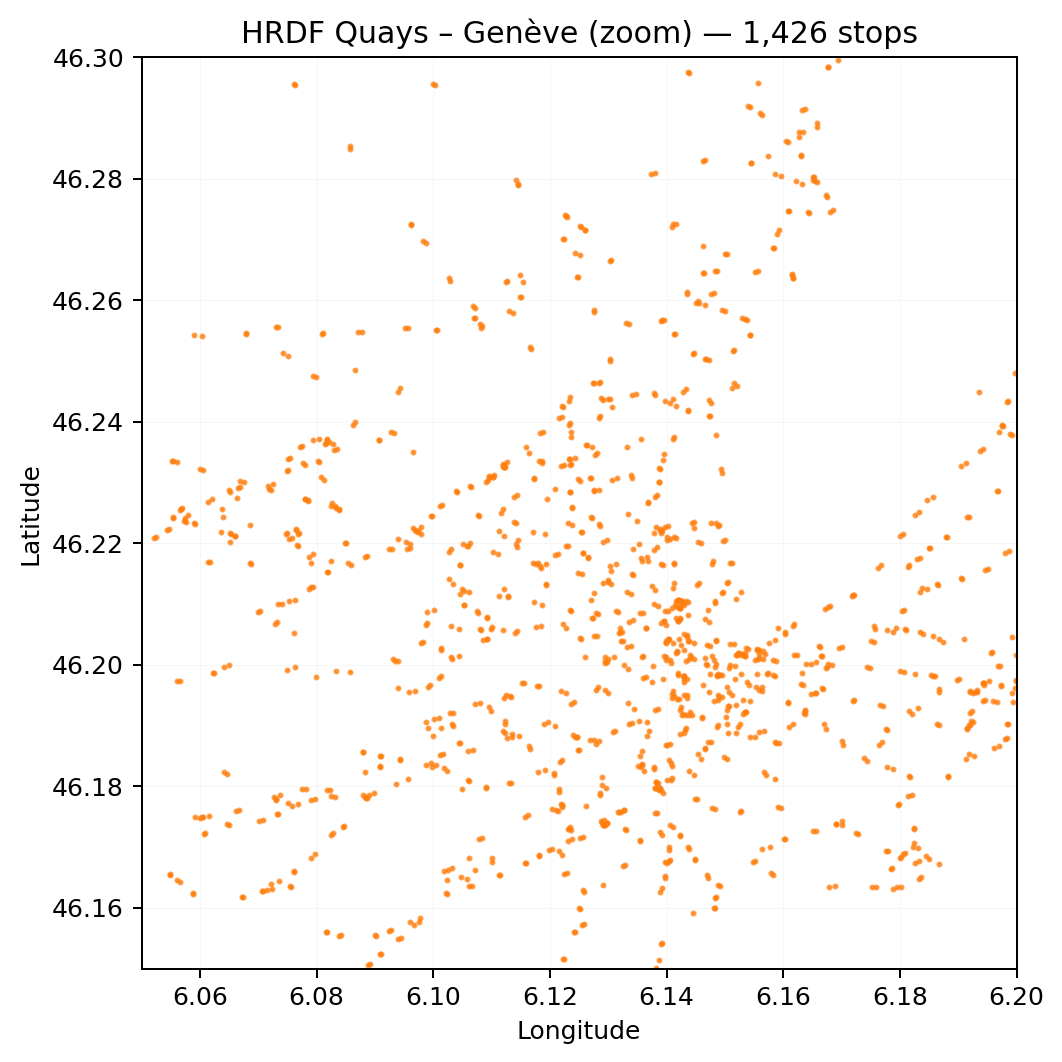
\includegraphics[width=.6\linewidth]{figures/plots/hrdf_quays_geneva.png}
  \caption[Quais HRDF – Genève]{Quais HRDF – zoom Genève.}
\end{figure}

\begin{figure}[h]
  \centering
  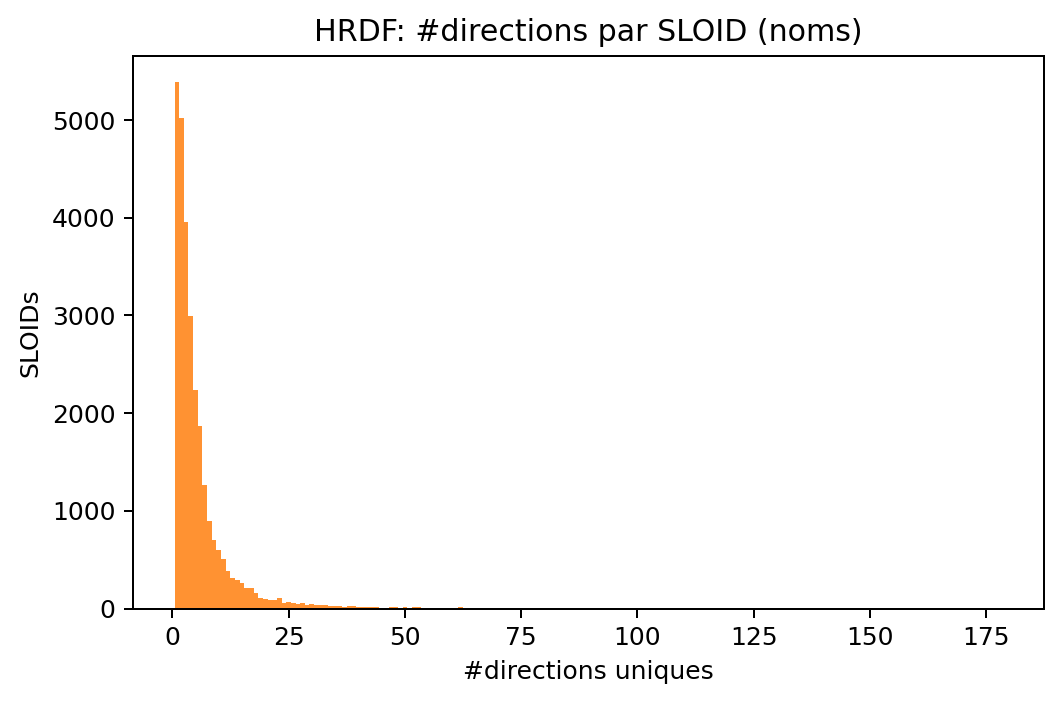
\includegraphics[width=.7\linewidth]{figures/plots/hrdf_directions_per_sloid.png}
  \caption{HRDF: distribution du nombre de \textit{directions (noms)} par SLOID.}
\end{figure}

\section{Comparaison GTFS et HRDF (couverture SLOID)}
\begin{itemize}
  \item GTFS: \textit{\(32\,248\)} SLOIDs\,; HRDF: \textit{\(28\,757\)} SLOIDs.
  \item Intersection: \textit{\(12\,206\)}\,; GTFS seulement: \textit{\(20\,043\)}\,; HRDF seulement: \textit{\(16\,551\)}.
\end{itemize}

\begin{figure}[h]
  \centering
  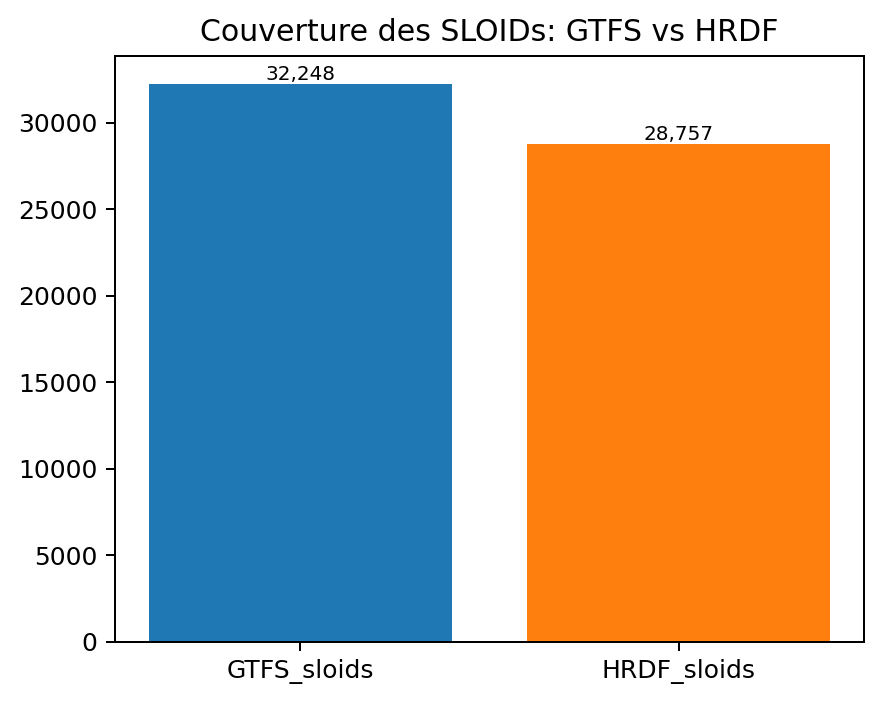
\includegraphics[width=.65\linewidth]{figures/plots/sloid_coverage_gtfs_hrdf.png}
  \caption[Couverture SLOID: GTFS vs HRDF]{Couverture SLOID: GTFS vs HRDF.}
\end{figure}

\begin{figure}[h]
  \centering
  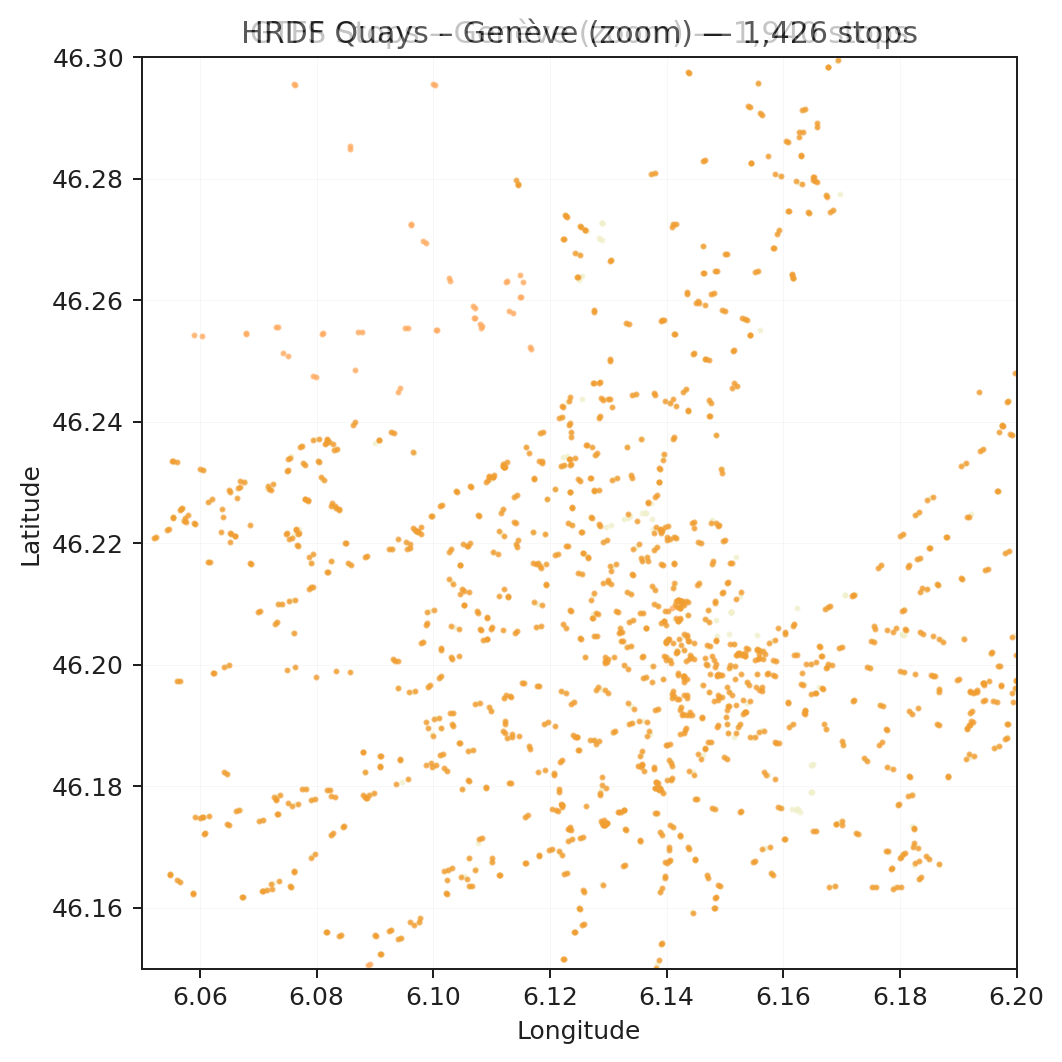
\includegraphics[width=.65\linewidth]{figures/plots/gtfs_hrdf_geneva_overlay.png}
  \caption[GTFS et HRDF à Genève]{GTFS et HRDF sur la même zone (Genève) — superposition aux mêmes limites spatiales.}
  \label{fig:gtfs_hrdf_geneva_overlay}
\end{figure}

\paragraph{Lien avec la suite.} Ces statistiques motivent notre \textit{route matching} (Chapitre~4) qui combine GTFS (identifiants \texttt{route\_id}/\texttt{direction\_id}) et HRDF (chaînes \textit{nom}/\textit{UIC}) afin d’optimiser précision et couverture.

\section{Chaîne d’acquisition et de prétraitement (vue d’ensemble)}
Le pipeline d’ingestion et de préparation des données est centralisé dans le module \texttt{get\_atlas\_data.py}. Il orchestre le téléchargement, le filtrage et l’agrégation des sources amont pour produire des artefacts compacts, déterministes et immédiatement consommables par la chaîne de \textit{matching}. Ses responsabilités principales sont:
\begin{enumerate}
  \item \textbf{ATLAS — acquisition et filtrage}: téléchargement du CSV le plus récent; restriction à la Suisse (\texttt{uicCountryCode = 85}); conservation des lignes avec coordonnées WGS84; écriture dans \texttt{data/raw/stops\_ATLAS.csv}.
  \item \textbf{GTFS — intégration (optimisée)}: extraction du ZIP; parcours en flux de \texttt{stop\_times.txt} en deux passes pour (i) identifier les trajets pertinents et les terminus suisses par trajet, (ii) dédupliquer \((\texttt{stop\_id},\texttt{route\_id},\texttt{direction\_id})\); jointure minimale avec \texttt{trips.txt} et \texttt{routes.txt}; appariement des arrêts GTFS aux SLOIDs ATLAS; écriture dans \texttt{data/processed/atlas\_routes\_gtfs.csv}.
  \item \textbf{HRDF — intégration (optimisée)}: extraction du ZIP; parsing ciblé de \texttt{GLEISE\_LV95} pour relier chaque \texttt{sloid} aux paires \((\text{UIC}, \#\text{ref})\) nécessaires; extraction des directions dans \texttt{FPLAN} (premier/dernier arrêt) avec résolution des noms via \texttt{BAHNHOF}; écriture dans \texttt{data/processed/atlas\_routes\_hrdf.csv}.
\end{enumerate}

\begin{figure}[h]
  \centering
  
\includegraphics[width=.82\linewidth]{diagram.pdf}
  \caption[Vue d’ensemble du pipeline]{Vue d’ensemble: acquisition (ATLAS/GTFS/HRDF) \(\to\) filtrage/streaming \(\to\) artefacts compacts pour la chaîne de \textit{matching}.}
\end{figure}

\subsection{Flux détaillé}
\paragraph{ATLAS.} Téléchargement depuis \textit{opentransportdata.swiss}, filtrage \texttt{uicCountryCode=85}, suppression des coordonnées manquantes. Résultat: référentiel des arrêts (SLOIDs) et attributs essentiels.

\paragraph{GTFS (streaming en deux passes).} Plutôt que de matérialiser un \texttt{DataFrame} \texttt{stop\_times} géant, nous effectuons deux passes en flux:
\begin{itemize}
  \item \textit{Passe 1}: identification des \texttt{trip\_id} desservant des arrêts suisses et calcul des terminus suisses par trajet (min/max \texttt{stop\_sequence}); puis chargement \emph{filtré} de \texttt{trips.txt} et \texttt{routes.txt}.
  \item \textit{Passe 2}: déduplication de \((\texttt{stop\_id},\texttt{route\_id},\texttt{direction\_id})\) et construction de chaînes directionnelles \enquote{\textit{Premier} $\to$ \textit{Dernier}} au niveau \texttt{route\_id}.
\end{itemize}
L’appariement \texttt{stop\_id} \(\leftrightarrow\) \texttt{sloid} s’appuie sur \texttt{uic\_number} et \texttt{designation} (avec normalisation des références locales \enquote{10000/10001} \(\to\) \enquote{1/2}).

\paragraph{HRDF (deux passes ciblées avec gardes rapides).} \texttt{GLEISE\_LV95} est parcouru avec des filtres \emph{très bon marché} (présence de \#, préfixe UIC à 7 chiffres, motif \enquote{ch:1:sloid:}) avant toute découpe. \emph{Passe 1}: découverte des paires \((\text{UIC}, \#\text{ref})\) par \texttt{sloid}. \emph{Passe 2}: collecte \emph{uniquement} des affectations de trajets dont la paire \((\text{UIC}, \#\text{ref})\) est requise. Les directions sont ensuite reconstruites via \texttt{FPLAN} et les noms d’arrêt de \texttt{BAHNHOF}.

\section{Principes d’ingénierie et d’optimisation}
Nos choix garantissent scalabilité et déterminisme:
\begin{itemize}
  \item \textbf{Streamer plutôt que matérialiser}: passes linéaires avec états compacts au lieu de gros \texttt{DataFrame}s temporaires.
  \item \textbf{Filtrer tôt et souvent}: réduire très tôt le périmètre (p. ex. \texttt{stop\_id} suisses commençant par \texttt{85}).
  \item \textbf{Parsing ciblé}: gardes substring à coût constant pour éviter \texttt{split()} et validations sur des lignes hors-scope.
  \item \textbf{Sorties déterministes}: mêmes résultats que les implémentations antérieures, afin d’isoler les améliorations aux seuls aspects performance/robustesse.
\end{itemize}

\section{Optimisations et résultats expérimentaux}
\subsection{Ingestion GTFS — streaming en deux passes}
\textbf{Problème.} La concaténation/filtration globale de \texttt{stop\_times} gonfle la mémoire et renchérit les fusions avec \texttt{trips}/\texttt{routes}.

\textbf{Solution.} Deux passes en flux (cf. supra), dédupliquant directement \((\texttt{stop\_id},\texttt{route\_id},\texttt{direction\_id})\) et construisant les directions au fil de l’eau.

\textbf{Impact.} Sur un échantillon \(2\%\), la mémoire de crête diminue de plus de moitié à sorties identiques. Plus lent sur un minuscule échantillon (surcoût fixe), le schéma \emph{scale} bien mieux en plein volume car il évite la matérialisation et les \textit{joins} coûteux.

\begin{table}[h]
  \centering
  \begin{tabular}{lrrr}
    \toprule
    \textbf{Mode} & \textbf{Temps (s)} & \textbf{Pic RSS $\Delta$ (MB)} & \textbf{Lignes} \\
    \midrule
    Baseline (2\%) & 20.17 & 275.4 & 8\,961 \\
    Streaming (2\%) & 43.28 & 123.7 & 8\,961 \\
    \bottomrule
  \end{tabular}
  \caption[Bench GTFS (2\%)]{Bench ingestion GTFS sur 2\%: fortes économies mémoire, sorties identiques; en plein volume, le streaming évite les \textit{joins} lourds.}
  \label{tab:gtfs-bench-ch1}
\end{table}

\paragraph{Pourquoi le streaming gagne.} Les surcoûts fixes (deux passes, états par \textit{chunk}) pèsent sur petit échantillon. À l’échelle, c’est la matérialisation initiale et les fusions massives qui dominent le coût; le streaming les supprime.

\subsection{Parsing HRDF — deux passes ciblées avec gardes}
\textbf{Problème.} \texttt{GLEISE\_LV95} est volumineux; découper/valider chaque ligne gaspille du CPU et conserver des mappages larges consomme de la mémoire.

\textbf{Solution.} Gardes substring rapides + deux passes ciblées: (1) découvrir \((\text{UIC}, \#\text{ref})\) par \texttt{sloid}, (2) ne conserver que les affectations utiles, puis reconstruire les directions via \texttt{FPLAN}/\texttt{BAHNHOF}.

\textbf{Impact.} Sur 2\,000 sloids, mêmes résultats, temps nettement réduit et surcoût mémoire négligeable.

\begin{table}[h]
  \centering
  \begin{tabular}{lrr}
    \toprule
    \textbf{Mode} & \textbf{Temps (s)} & \textbf{Pic RSS $\Delta$ (MB)} \\
    \midrule
    Baseline & 26.18 & 1745.0 \\
    Optimisé (deux passes + gardes) & 14.54 & $\approx$ 0.0 \\
    \bottomrule
  \end{tabular}
  \caption[Bench HRDF (2k sloids)]{Parsing HRDF: bench sur 2k sloids.}
  \label{tab:hrdf-bench-ch1}
\end{table}

\section{Reproductibilité et exécution}
\noindent\textbf{Instantané.} Sauf mention contraire, toutes les statistiques/cartes reposent sur l’instantané du \textbf{11 août 2025} (cf. tête de chapitre).\medskip

\noindent\textbf{Scripts.} Les scripts de génération des figures et des métriques sont archivés sous \texttt{memoire/scripts\_used/}. Pour régénérer les artefacts GTFS/HRDF:

\begin{cmdbox}
python3 get_atlas_data.py
\end{cmdbox}

\noindent\textbf{Sorties produites.}
\begin{itemize}
  \item \texttt{data/raw/stops\_ATLAS.csv} — référentiel d’arrêts ATLAS filtré.
  \item \texttt{data/processed/atlas\_routes\_gtfs.csv} — relations arrêt–route–direction et chaînes directionnelles.
  \item \texttt{data/processed/atlas\_routes\_hrdf.csv} — lignes \texttt{sloid}–direction (noms et UIC) issues d’HRDF.
\end{itemize}

